\documentclass[tikz,border=2mm,12pt]{standalone}

\begin{document}
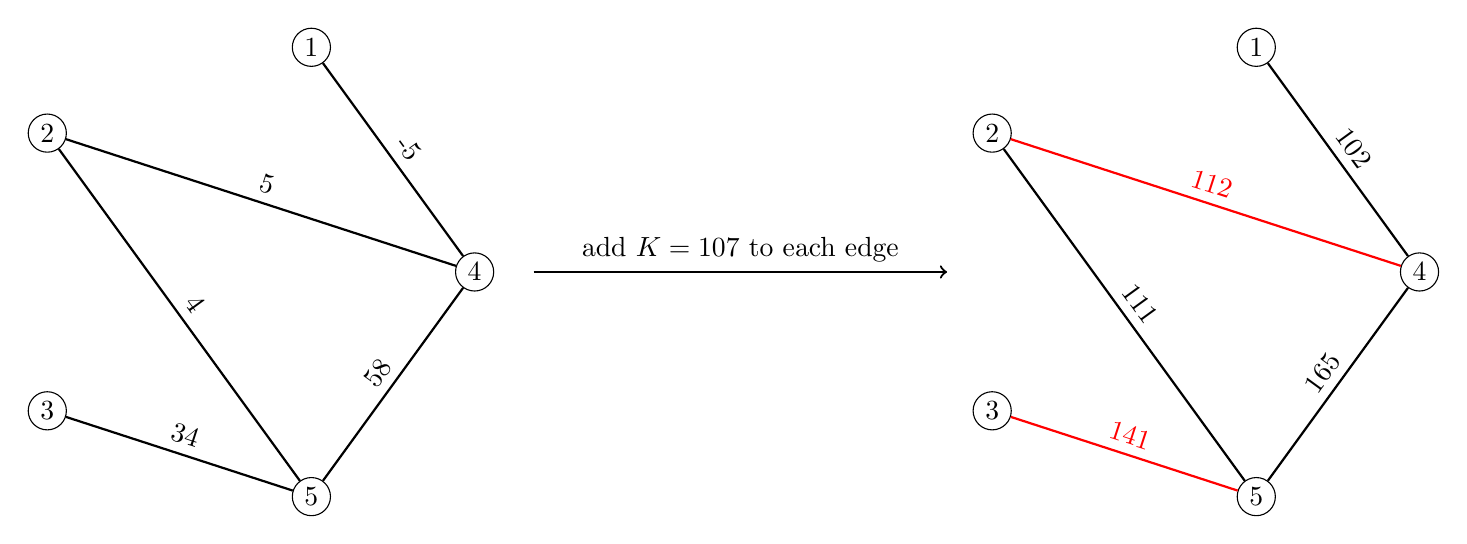
\begin{tikzpicture}[scale=1.5]
    % Define nodes with labels for the first graph
    \foreach \i/\label in {1/1, 2/2, 3/3, 4/5, 5/4}
    \node[circle, draw, inner sep=2pt] (node\i) at (\i*72:2cm) {\label};

    % Define edges with weights and colors for the first graph
    \foreach \source/\dest/\weight/\edgecolor in {1/5/-5/black, 2/5/5/black, 2/4/4/black, 3/4/34/black, 5/4/58/black}
    \draw[thick, \edgecolor] (node\source) -- node[midway, above, sloped] {\weight} (node\dest);

    % Draw an arrow and label
    \draw [->,thick] (2.5,0) -- node[above] {add $K=107$ to each edge} (6,0);

    % Shift the position for the second graph
    \begin{scope}[xshift=8cm]
        % Define nodes with labels for the second graph
        \foreach \i/\label in {1/1, 2/2, 3/3, 4/5, 5/4}
        \node[circle, draw, inner sep=2pt] (node\i) at (\i*72:2cm) {\label};

        % Define edges with weights and colors for the second graph
        \foreach \source/\dest/\weight/\edgecolor in {1/5/102/black, 2/5/112/red, 2/4/111/black, 3/4/141/red, 5/4/165/black}
        \draw[thick, \edgecolor] (node\source) -- node[midway, above, sloped] {\weight} (node\dest);

    \end{scope}
\end{tikzpicture}
\end{document}
